\documentclass[dvipdfmx]{ampbt}
%% compile: platex thesis.tex && bibtex thesis && platex thesis.tex && platex thesis.tex && dvipdfmx thesis.dvi

%% クラスオプション:
%% chapter:   \chapterコマンドを使用可能にする(jsbook (report) を使う).
%% duplexing: 両面印刷用の PDF を出力する.
%% その他 jsclasses に指定可能なオプションが指定できます(そのまま渡される).

%% 報告書の題目 %%%%%%%%%%%%%%%%%%%%%%%%%%%%%%%%%%%%%%%%%%%%%%%%%%%%%%%%%%%%%%%%%
\title{Friend-to-friendネットワークにおける} % 題目1行目
      {効率的な分散ルーティング}                         % 題目2行目
      {}                                         % 題目3行目
%% 指導教員 %%%%%%%%%%%%%%%%%%%%%%%%%%%%%%%%%%%%%%%%%%%%%%%%%%%%%%%%%%%%%%%%%%%%%
\supervisors{宮崎修次}{講師}    % 指導教員1人目 {氏名}{職名}
            {}{}    % 指導教員2人目 {氏名}{職名}
            {}{}                % 指導教員3人目 {氏名}{職名}
%% 入学年月 %%%%%%%%%%%%%%%%%%%%%%%%%%%%%%%%%%%%%%%%%%%%%%%%%%%%%%%%%%%%%%%%%%%%%
\entrancedate{24}{4}            % {年(平成)}{月}
%% 著者氏名 %%%%%%%%%%%%%%%%%%%%%%%%%%%%%%%%%%%%%%%%%%%%%%%%%%%%%%%%%%%%%%%%%%%%%
\author{高橋}{彰}             % {姓}{名}
%% 提出日 %%%%%%%%%%%%%%%%%%%%%%%%%%%%%%%%%%%%%%%%%%%%%%%%%%%%%%%%%%%%%%%%%%%%%%%
\submissiondate{29}{1}{XX}      % {年(平成)}{月}{日}
%% 提出年度 %%%%%%%%%%%%%%%%%%%%%%%%%%%%%%%%%%%%%%%%%%%%%%%%%%%%%%%%%%%%%%%%%%%%%
\submissionjay{28}              % {年度(平成)}
%% 摘要 %%%%%%%%%%%%%%%%%%%%%%%%%%%%%%%%%%%%%%%%%%%%%%%%%%%%%%%%%%%%%%%%%%%%%%%%%
\abstract{%
  本研究では, F2Fネットワークトポロジーのスモール・ワールド性を利用し, 効率的かつ非中央集権的なルーティングを実現するための手法を提起する. 
}
%% パッケージの読み込みや自分用のマクロの定義 %%%%%%%%%%%%%%%%%%%%%%%%%%%%%%%%%%%
\usepackage{amsmath,amssymb}
\newcommand{\rme}{\mathrm{e}}

%% 出力の制御 %%%%%%%%%%%%%%%%%%%%%%%%%%%%%%%%%%%%%%%%%%%%%%%%%%%%%%%%%%%%%%%%%%%

%% 本文を出力しない場合,次の行をコメントアウトして下さい.
% \outputbodyfalse

%% 末尾に表紙,背表紙を出力しない場合,次の行をコメントアウトして下さい.
% \outputcoverfalse

%% 末尾に提出用摘要を出力しない場合,次の行をコメントアウトして下さい.
% \outputabstractforsubmissionfalse

%% ampbt.cls では表紙等の作成のために geometry パッケージを使用しているため,本文
%% のレイアウトを変えるために \usepackage[...]{geometry} とすると Option clash が
%% 発生します.何らかの理由で本文のレイアウトを変更したい場合は \geometry{...} を
%% 使用して下さい.
%% また,jsclasses を使用しているため,例えば 3cm を指定したい場合は 3truecm と書
%% く必要があります.
% \geometry{hmargin=3truecm,vmargin=2truecm}

\begin{document}
\ifoutputbody
%% 中表紙,摘要,目次 %%%%%%%%%%%%%%%%%%%%%%%%%%%%%%%%%%%%%%%%%%%%%%%%%%%%%%%%%%%
\makeinsidecover                % 中表紙
\makeabstract                   % 摘要
\maketoc                        % 目次
\setcounter{page}{1}            % 本文のページ番号を1から始める
%% 本文 %%%%%%%%%%%%%%%%%%%%%%%%%%%%%%%%%%%%%%%%%%%%%%%%%%%%%%%%%%%%%%%%%%%%%%%%%
\section{序論}
近年インターネットを介したコミュニケーションまたは出版は, 我々の生活において大きな位置を占めるようになってきた. それに伴いユーザーのプライバシー保護を重視したコミュニケーションツールの実装に対する需要が非常に高まっている. その要因として, 例えば近年ではエドワード・スノーデンによって公に明らかにされたアメリカ国家安全保障局(NSA)による大規模な大衆監視が挙げられる. \newline
\ \ 特定の企業や団体が中央集権的に管理する情報共有方式はこのような監視・漏洩のリスクが高いため, 非中央集権的な情報共有を実現するためのアプローチとしてP2P方式が頻繁に採用される. P2Pは中心的な管理者を持たない分散的なオーバーレイネットワークであり, 一般的なクライアント-サーバー方式と比較して負荷分散, スケーラビリティ, 匿名性, 耐障害性等の点で優れている\cite{lua2005survey}. そしてP2P方式の中でも特にピアの匿名性・プライバシー保護を重視したものはfriend-to-friend(F2F)\cite{bricklin2000friend}, またはDarknet\cite{clarke2010private}と呼ばれる. F2F方式においてネットワーク上の各ノードは, 信頼のおける特定ノードとのみ通信するため, Chord\cite{stoica2001chord}などの分散ハッシュテーブル(DHT)方式とは異なり, ソフトウェアによって動的にネットワーク構造を最適化することはできず, ネットワーク構造は常に現実の信頼関係ネットワークの部分グラフに対応する. そしてネットワーク上で隣接していないノード同士がデータの送受信を行うためにはいずれかのノードが「知り合いの知り合い」を辿って他方のノードに到達するための経路を探索する必要性が生じる\cite{roos2016dealing}.\newline
\ \ F2Fオーバーレイネットワークの最も代表的な実装例は, Freenet\cite{clarke2001freenet}のDarknetモード\cite{clarke2010private}であり, 基本的なプロトコルはSandberg\cite{sandberg2006distributed}が2006年に提案した手法に基づいている. Freenetでは, 信頼関係のネットワークがスモールワールド性を持つと仮定し, 単純なgreedyルーティング (各ノードは隣接ノード中, 最もターゲットに近いノードを次ノードとして選択) により, $O(\log^2 n)$のホップ数でルーティングを可能にするKleinbergのスモールワールドネットワークモデル\cite{kleinberg2000small}に基づいている. \newline
\ \ ただしFreenetには未だ様々な問題点が残っている. 第一にSandbergが提案した手法では, Kleinbergモデルが依拠している「格子上で最も近距離にいるノード同士は必ずエッジを持つ」という仮定を決定論的に満たすことができないため, Freenetの実装においてはgreedyルーティングの代わりにdistance-directed depth-first search ($D^2$-$DFS$)が採用されている. しかしこの$D^2$-$DFS$アルゴリズムが$O(\log^2 n)$のホップ数を達成することができないことはRoos, Strufeらにより解析的に証明された\cite{roos2012provable} \cite{roos2016dealing}\cite{roos2016analyzing}. またFreenetでは, ノード集合$V$から座標空間$C= [0,1)$への「埋め込み」(embedding) $\phi: V \to C$を生成するMetropolis-Hastingsアルゴリズムの一環としてノード同士が座標(Freenetの実装ではID)を交換する操作を反復するが, この際悪意のあるノードが虚偽のID報告を繰り返すことにより, ノードが格子上に偏在し, 結果的にルーティングの効率性が低下するというPitch black attack\cite{evans2007routing}などの深刻な脆弱性が指摘されている. よってFreenetのDarkenetモードは効率性や頑健性の面で問題点が残り, 現在もそれらを解決するための研究が続けられている. \newline
\ \ 本研究では, 以上に挙げられたFreenetの問題点のうちルーティングの効率性に着目する. 今回我々はSimsek, Jensenらによって提案されたルーティングアルゴリズム, expected-value navigation (EVN)\cite{csimcsek2008navigating}をFreenetプロトコルに適用可能な形に修正することにより, 埋め込みの不正確さと, 現実のネットワークに存在する多数のリーフノードに対しロバストなルーティングアルゴリズムを提起する.

 \section{先行研究}
   \subsection{P2Pネットワーク}
   \subsection{複雑ネットワーク}
   \subsection{Kleinbergモデル}
   \subsection{Greedy embedding}
   \subsection{Freenetプロトコル: 埋め込みとルーティング}
   \subsection{EVN: Expected-value navigation}
\if0
\cite{clarke2001freenet}
\cite{sandberg2006distributed}
\cite{sandberg2006evolution}
\cite{sandberg2008neighbor}
\cite{mogren2008adaptive}
\cite{evans2007routing}
\cite{clarke2010private}
\cite{schiller2011attack}
\cite{roos2012provable}
\cite{roos2013contribution}
\cite{roos2016dealing}
\cite{hofer2013greedy}
\cite{roos2016anonymous}
\cite{roos2016analyzing}
\cite{kleinberg2000small}
\cite{csimcsek2008navigating}
\cite{serrano2008self}
\cite{boguna2009navigating}
\cite{boguna2009navigability}
\cite{kleinberg2007geographic}
\cite{cvetkovski2009hyperbolic}
\cite{krioukov2010hyperbolic}
\cite{boguna2010sustaining}
\cite{papadopoulos2015network}
\cite{blasius2016efficient}
\cite{kleinberg2006complex}
\cite{huang2014navigation}
\cite{van2010graph}
\fi

\section{問題設定}
TBD
\section{提案手法}
TBD
   \subsection{ネットワークモデル}
   TBD
   \subsection{ルーティングアルゴリズム}
   TBD


\section{評価}
  \subsection{シミュレーション手法}
  TBD
  \subsection{シミュレーション結果}
\begin{figure}[htbp]
  \centerline{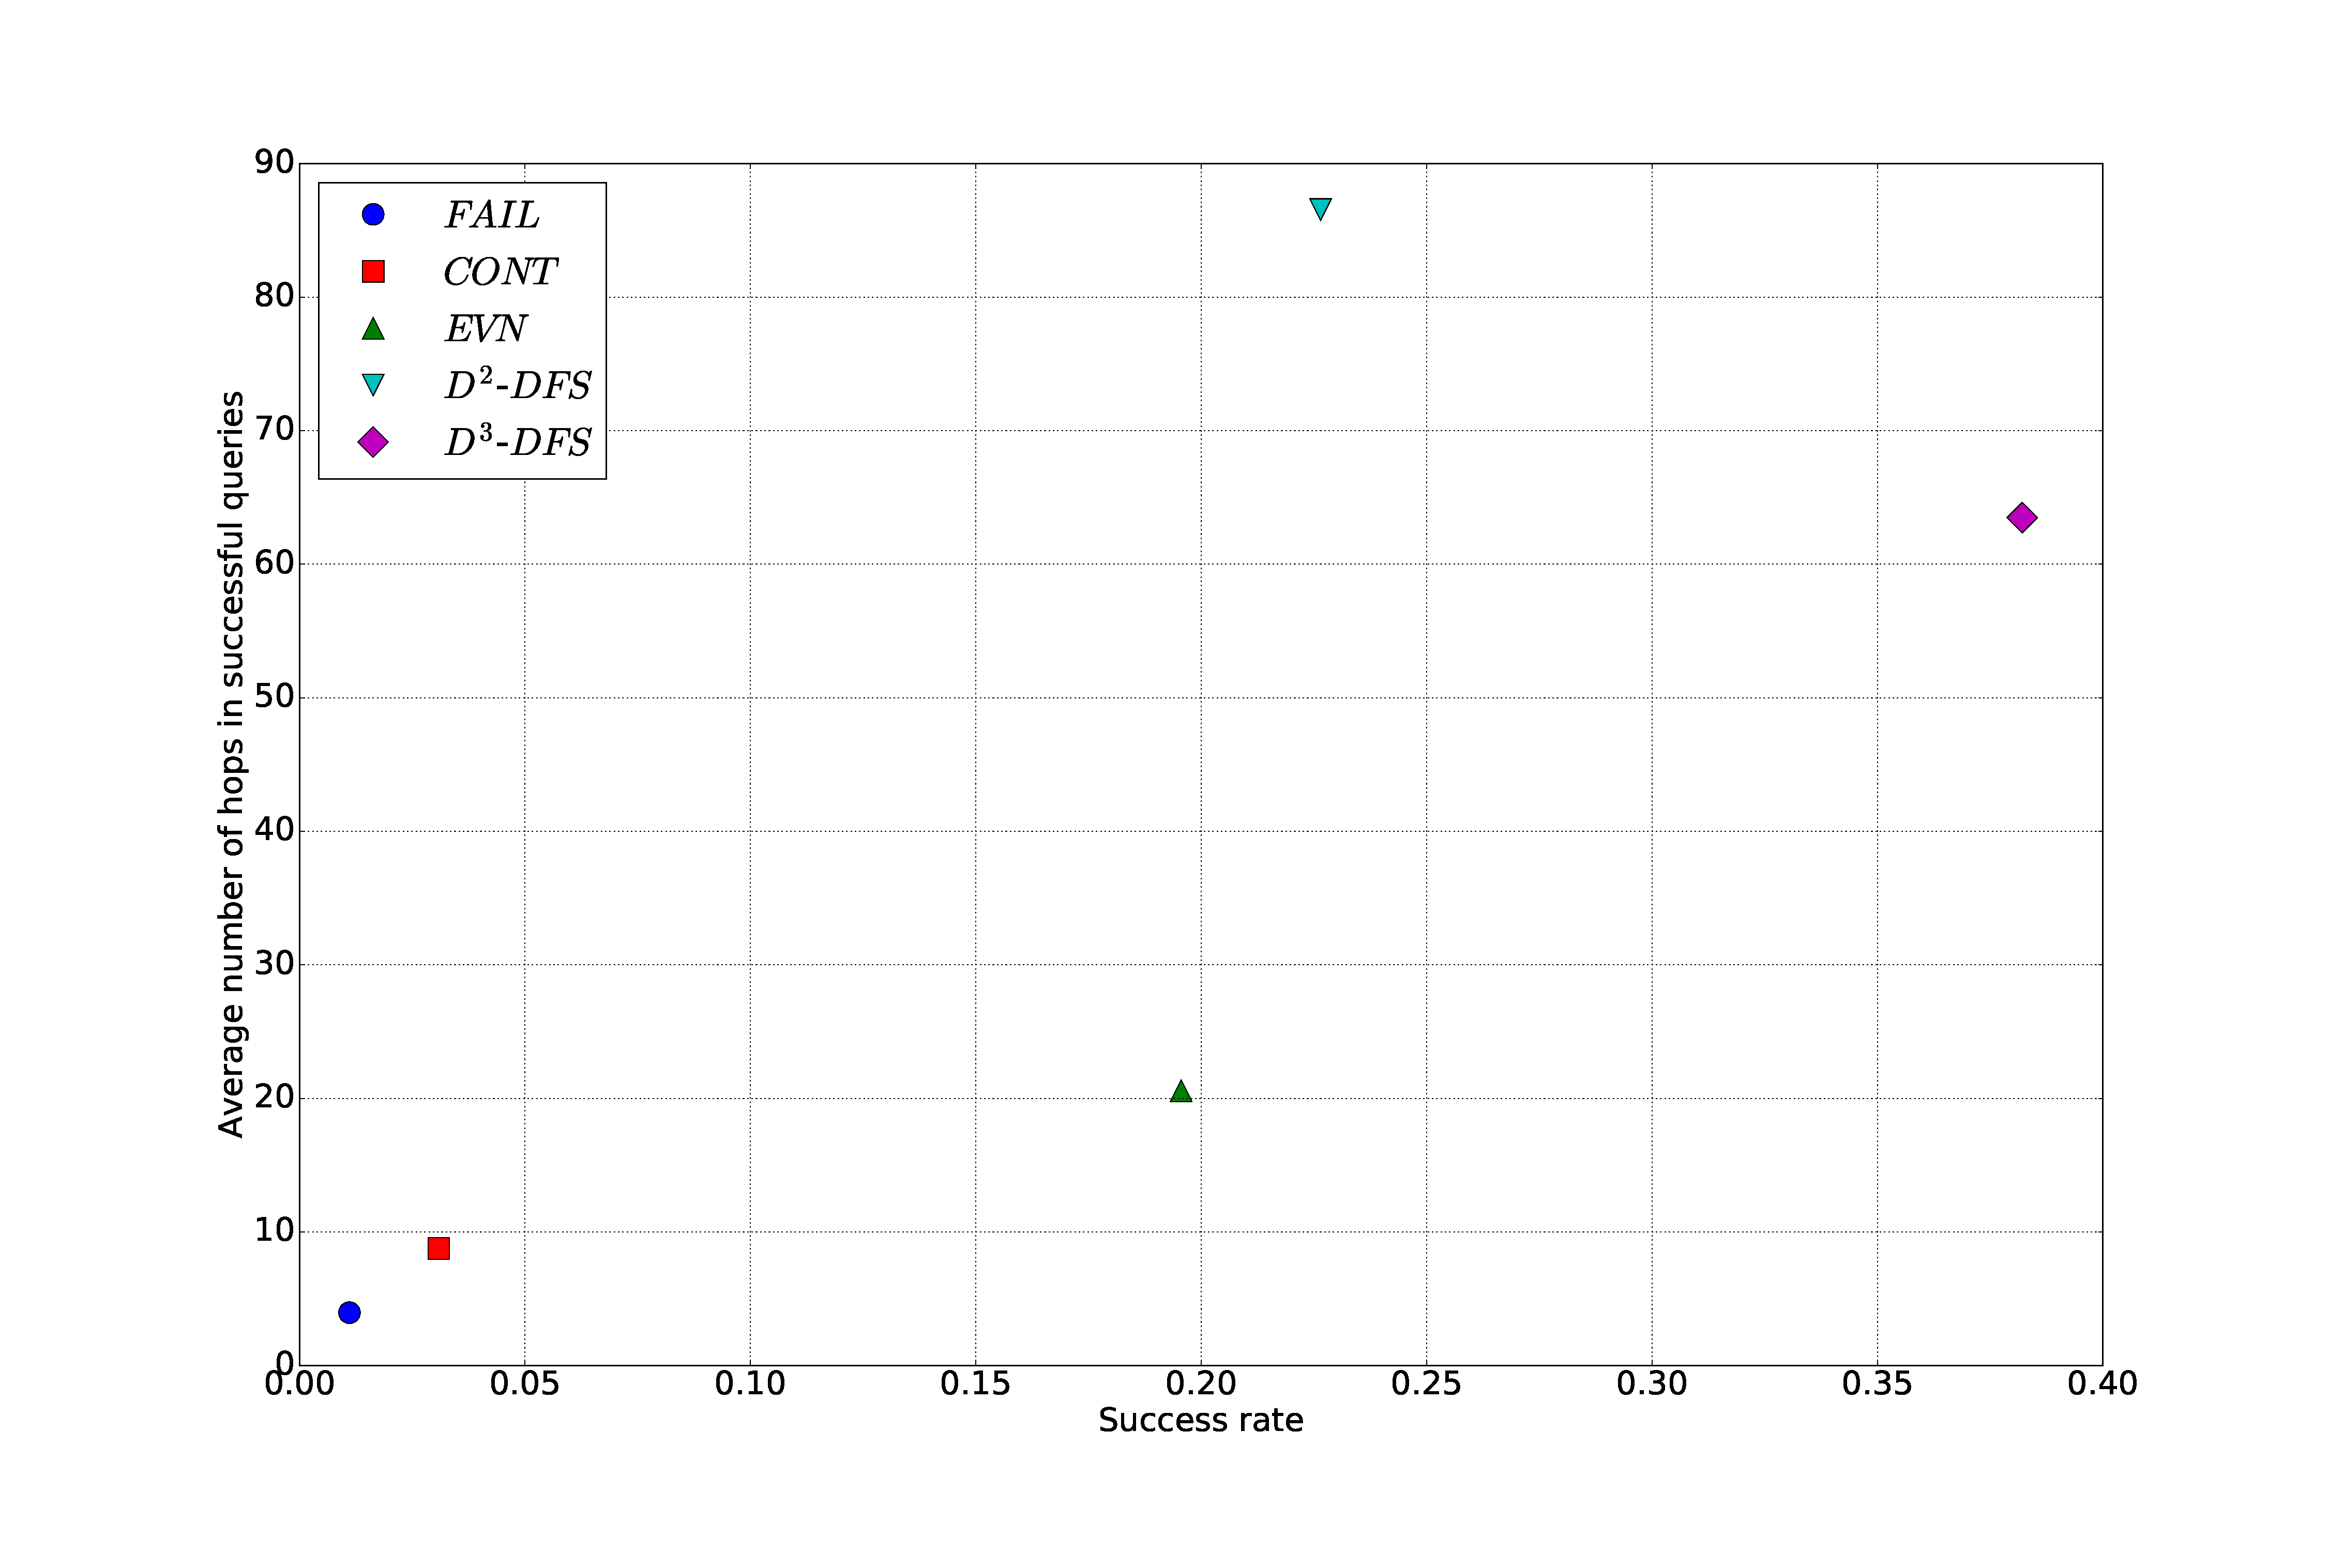
\includegraphics[width=120mm]{../fig/succ_hops_full.eps}}
  \caption{ID割り当て後のWeb of Trustネットワークにおける各ルーティングアルゴリズムの成功率と平均ホップ数}
  \label{fig:succ_hops_full}
\end{figure}

\section{結論と今後の展望}
TBD
%% 謝辞 %%%%%%%%%%%%%%%%%%%%%%%%%%%%%%%%%%%%%%%%%%%%%%%%%%%%%%%%%%%%%%%%%%%%%%%%%
\acknowledgment

%% 参考文献 %%%%%%%%%%%%%%%%%%%%%%%%%%%%%%%%%%%%%%%%%%%%%%%%%%%%%%%%%%%%%%%%%%%%%
\clearpage
\addcontentsline{toc}{section}{\refname} % 目次に参考文献を追加する.
                                         % chapter使用時は削除すること.

%% BibTeX 等を用いる場合は,上の thebibliography 環境を消してここに該当コードを
%% 挿入すること.
\bibliographystyle{ieeetr}
\bibliography{refs}


\clearpage
%% 付録 %%%%%%%%%%%%%%%%%%%%%%%%%%%%%%%%%%%%%%%%%%%%%%%%%%%%%%%%%%%%%%%%%%%%%%%%%
%% 付録は不要ならば削除してよい.
\appendix

\section{用語集}

\begin{table}[htbp]
  \caption{これは意味のない表です.}
  \centering
  \begin{tabular}{c|cc}
      &  A  &  B \\
    \hline
    C &  70 & 80 \\
    D & 100 &  0
  \end{tabular}
\end{table}

%% 本文ここまで %%%%%%%%%%%%%%%%%%%%%%%%%%%%%%%%%%%%%%%%%%%%%%%%%%%%%%%%%%%%%%%%%
\fi
\ifoutputcover
\evenclearpage
%% 表紙,背表紙,提出用摘要 %%%%%%%%%%%%%%%%%%%%%%%%%%%%%%%%%%%%%%%%%%%%%%%%%%%%%
\makecover                      % 表紙
\makespine[1]                   % 背表紙([] 内は出力枚数)
\makeinsidecover                % 中表紙
\fi
\ifoutputabstractforsubmission
\makeabstractforsubmission      % 提出用摘要
\fi
\end{document}
